The general approach to the design of \pol{} protocols has been mainly focused on the proof generation process, as seen in the multiple examples dissected in Chapter~\ref{sec:related-work}. Advancements made towards more distributed and decentralized solutions have highlighted the need for a comprehensive and detailed description of the protocol's entire range of requirements. To achieve an operable system that meets the demands of real-world applications, a phased strategy with a keen awareness of the intrinsic details, at every stage of the solution, is essential for providing a complete and coherent picture of the protocol's design. Therefore, we will attempt at the design of a \pol{} protocol that starts with an infrastructural foundation, and ends with a complete system~\textemdash~aiming to achieve the goal of proving one's location.

\begin{figure}[ht]
    \begin{center}
    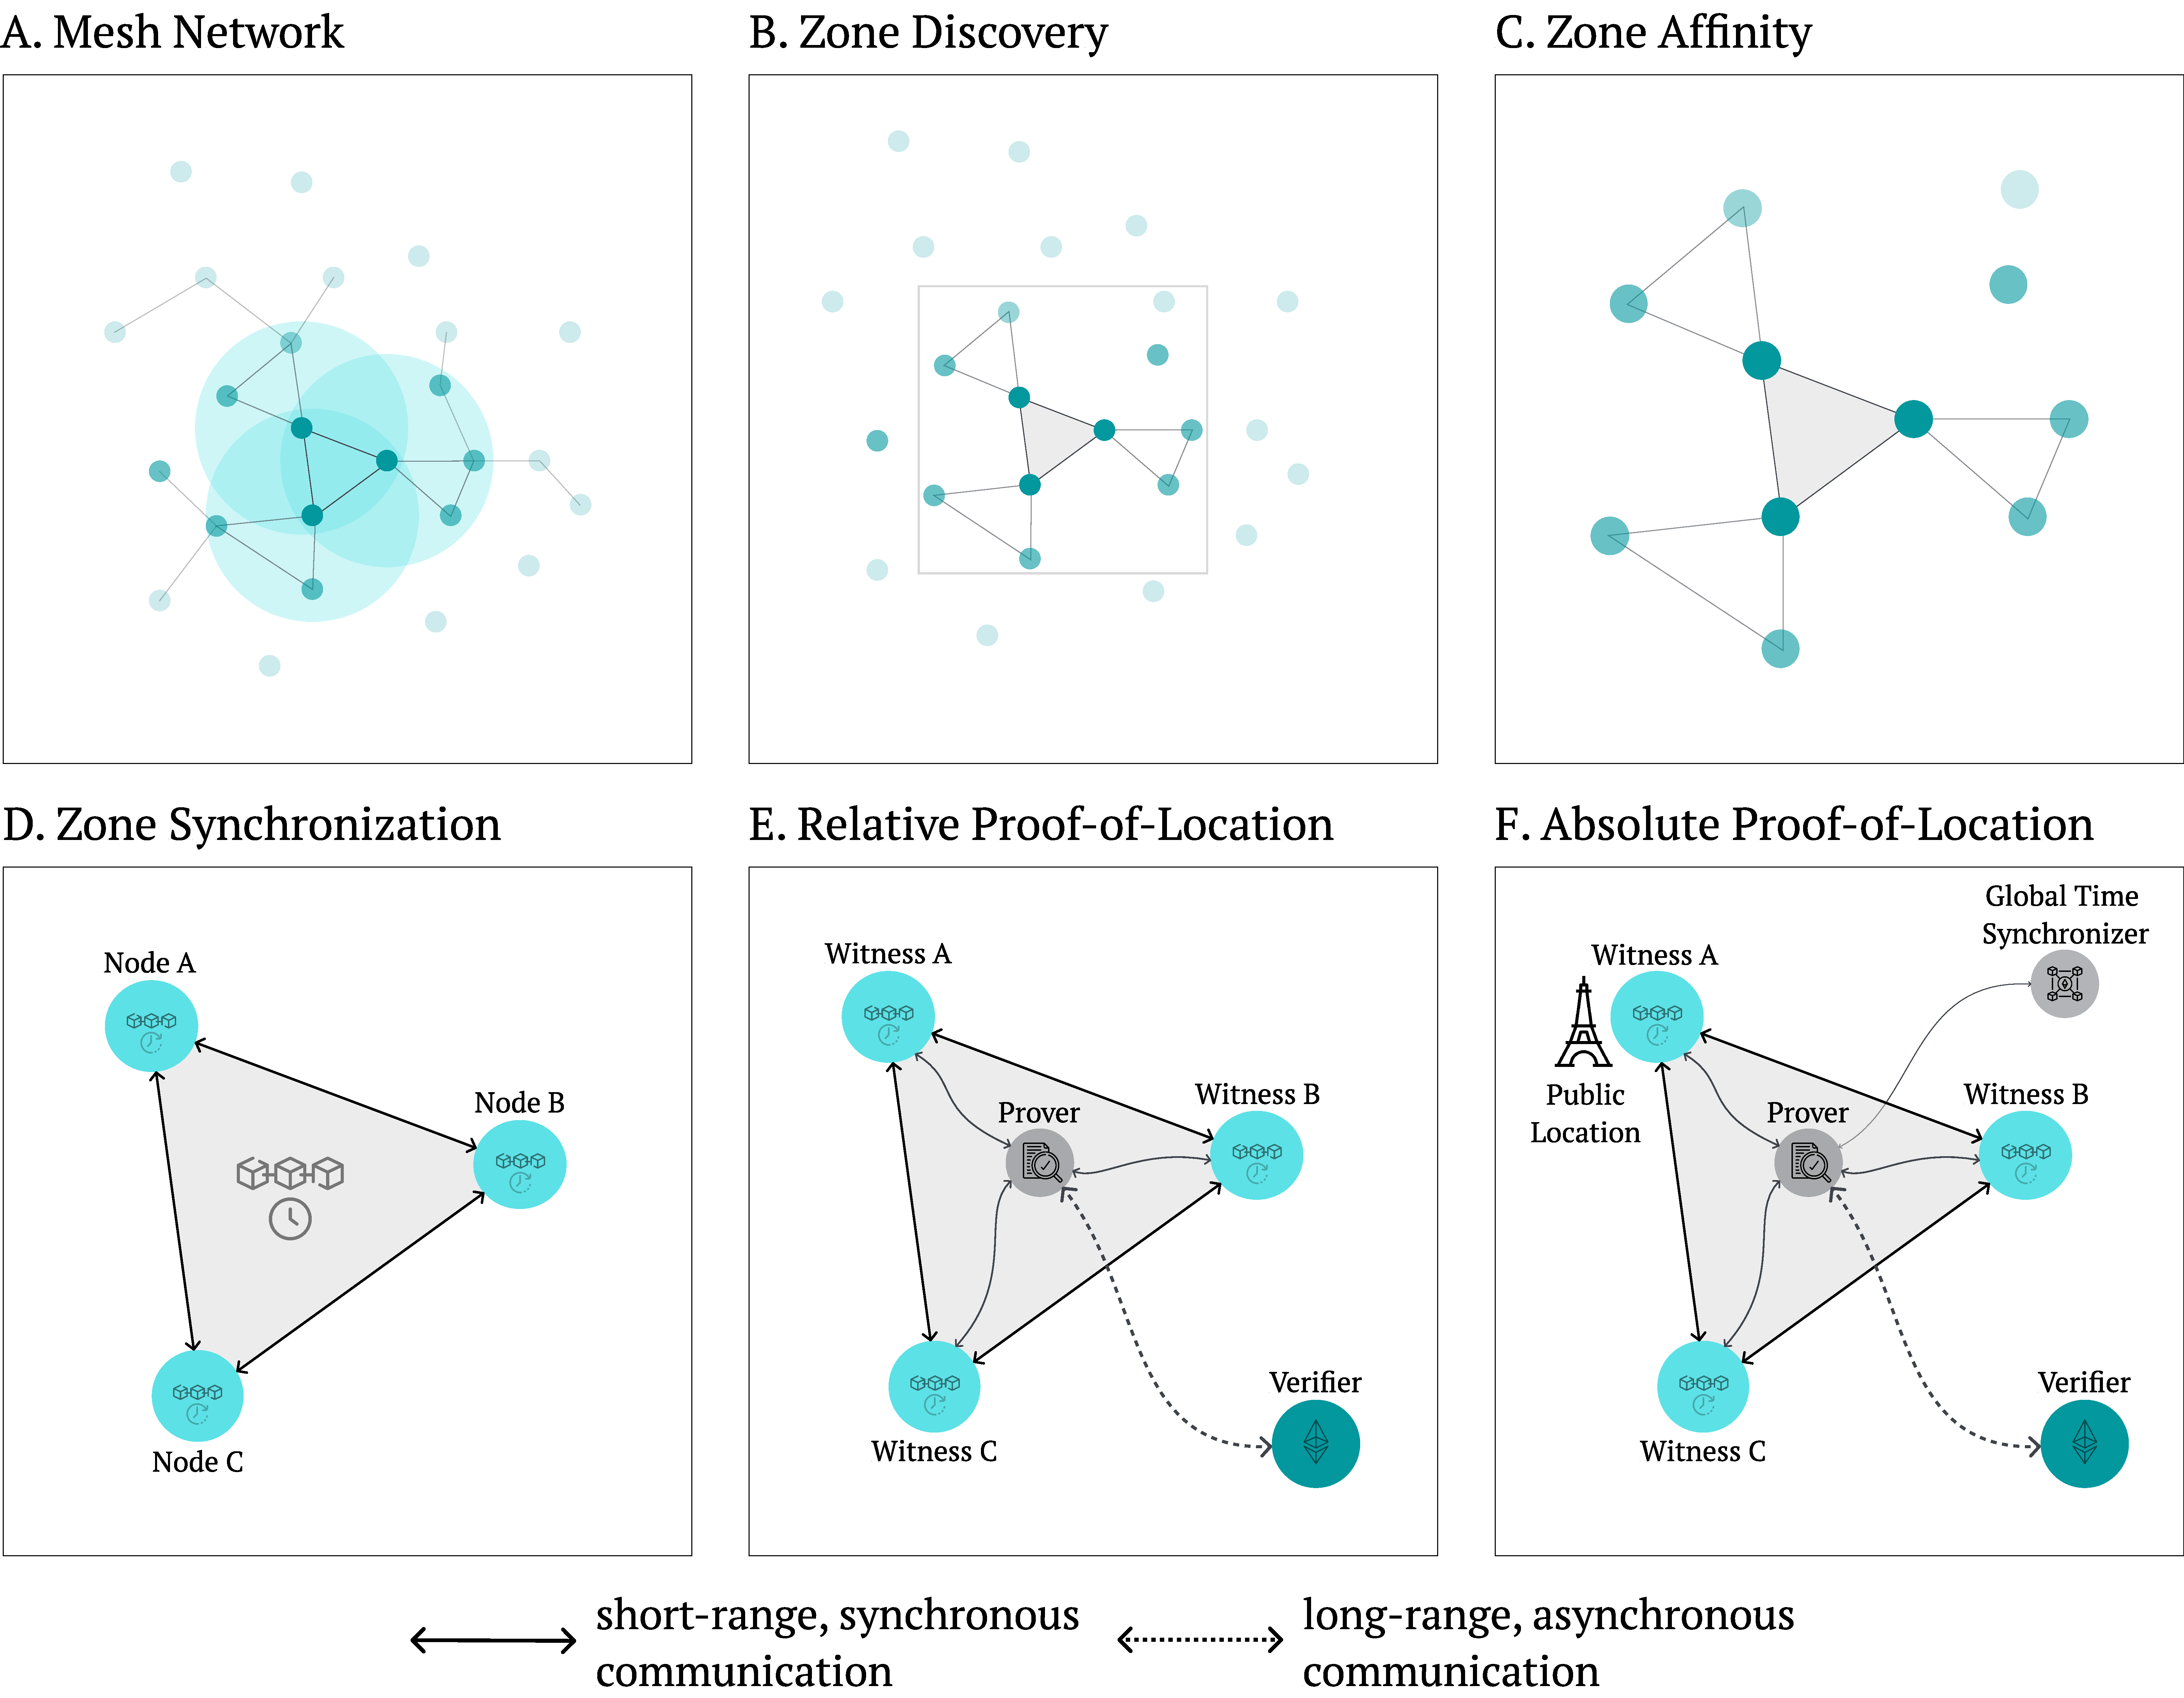
\includegraphics[width=0.9\textwidth]{overview-pol.pdf}
    \caption{A discretization attempt to capture the multiple steps of the protocol design, from a dynamic mesh topology, towards the ultimate goal of achieving Absolute \pol.}
    \label{fig:proof-of-location-overview}
    \end{center}
\end{figure}

The following sections will guide the reader through the multiple steps of the protocol's design. This journey, depicted in Figure~\ref{fig:proof-of-location-overview}, starts with the foundation layer of the system, powered by a dynamic and non-hierarchic Mesh Network topology. This topology should enable the network agents to communicate with each other in a peer-to-peer, short-ranged, and conveniently wireless fashion. The next step entails the nodes' neighbourhood establishment, eased by lower-layer routing protocols, leading to the eventual creation of fully connected zones of neighbours. Each node, however, may simultaneously belong to multiple zones, with the processes of zone affinity, zone switching, zone expanding, and, consequently, the overall configuration of the mesh topology being dictated by protocol requirements. Application-level incentives, in the lines of the ones envisioned in the FOAM protocol, may also take part in encouraging the formation of zones and growth of the network. The goal is to achieve a latticework of space and time, with zone-relative clock precision. Therefore, the next step is to establish, or derive, spatio-temporal zone synchronization. Space synchrony is accomplished with the assumptions regarding the short-ranged communication means. To achieve time synchrony, a clock synchronization mechanism is necessary. This mechanism not only ensures the synchronization of the witnesses' internal clocks, but can also enable zone-relative event serialization, via a strongly consistent consensus-based system. Moreover, by choosing and employing a Turing-complete consensus protocol, it becomes possible to execute more complex logic alongside these functionalities, for instance, with the deployment of smart contracts that potentiate the creation of decentralized and zone-relative location services. Nonetheless, the main aim is to achieve zone-relative time consciousness, to then enable spatio-temporal soundness and provide complete location proofs \cite{nasrulin2018robust}.

In the following sections, we will provide a more detailed analysis of these multiple steps. However, in the practical work, we will focus only on a subset of the entire problem. For the implementation of the \poc{} in Chapter~\ref{sec:proof-of-concept}, it is assumed that the processes of zone discovery and zone affinity management have already been accomplished, and the nodes have agreed to form a zone. The steps that follow the goal of achieving relative \pol{} are also left for future work.
